\documentclass[journal]{IEEEtran}

% Packages
\usepackage{amsmath}
\usepackage{graphicx}
\graphicspath{./Images/}
\usepackage[table,dvipsnames]{xcolor}
\usepackage{booktabs}
\usepackage{wrapfig}
\usepackage{float}
\usepackage{cite}
\usepackage{url}
\usepackage{tikz}
\usetikzlibrary{matrix,shapes,positioning,arrows,backgrounds}

% Drafting Utility Package
\usepackage{comment}

% Title
\title{A Comparative Study of Techniques for Addressing Class Imbalance in Machine Learning}

\author{Brandon Hosley, Capt, \textit{AFIT}%
	\thanks{Manuscript received May 16, 2023%
		%		; revised Month DD, YYYY.
}}

%\keywords{class imbalance, data-level methods, algorithm-level methods, hybrid methods, machine learning, performance evaluation}

% Document
\begin{document}
	
	\maketitle
	
	
	% Abstract
	\begin{abstract}
		Class imbalance is a pervasive challenge in machine learning, occurring when the distribution of classes in a dataset is significantly skewed. Traditional learning algorithms often struggle to accurately classify minority classes due to the dominance of majority classes. To address this issue, various techniques have been proposed to mitigate the impact of class imbalance on model performance. This paper presents a comparative analysis of different methods for handling class imbalance, aiming to provide insights into their effectiveness and suitability across a range of domains and datasets.
	\end{abstract}
	
	% Introduction
	\section{Introduction}
	\label{sec:introduction}
	Class imbalance is a pervasive challenge in machine learning, where certain classes within a dataset are significantly underrepresented compared to others. This disparity often leads to biased models that are less accurate in predicting minority class instances, resulting in suboptimal overall performance. In various real-world applications, such as fraud detection, medical diagnosis, and rare event prediction, the minority class is often more significant than the majority class. In critical domains, such as medical diagnoses, where the cost of false negatives is extremely high, failing to correctly identify instances of the minority class can have severe implications. Consequently, it is crucial to develop effective strategies that mitigate the impact of class imbalance on model performance.
	
	In recent years, researchers have proposed numerous techniques to address class imbalance and improve model performance. These methods can be broadly categorized into three main approaches: data-level methods, algorithm-level methods, and hybrid methods. Data-level methods focus on modifying the dataset itself by oversampling the minority class, undersampling the majority class, or generating synthetic samples. Algorithm-level methods aim to adapt existing machine learning algorithms or design new ones that are more robust to class imbalance. Hybrid methods combine data-level and algorithm-level techniques to leverage the advantages of both.
	
	Given the abundance of class imbalance handling methods, it becomes crucial to conduct a comparative analysis to understand their relative strengths and weaknesses. 
	% We evaluate the effectiveness of each method using a diverse set of real-world and synthetic datasets, encompassing various levels of class imbalance and problem complexities. 
	% Our assessment includes a thorough analysis of performance metrics, such as accuracy, precision, recall, F1-score, and area under the receiver operating characteristic curve (AUC-ROC), to provide a holistic understanding of the impact of each technique on model performance.
	By empirically evaluating these techniques on diverse datasets and considering different evaluation metrics, we can gain insights into their effectiveness, applicability, and trade-offs. This paper aims to bridge this gap by providing a comprehensive evaluation of 
	%state-of-the-art class imbalance handling methods.
	well-known class imbalance handling methods.
	
	By comparing and contrasting these methods, we aim to provide practitioners and researchers with valuable insights into the relative strengths and weaknesses of each technique. Moreover, our study intends to offer guidelines for selecting the most appropriate approach based on the specific characteristics of a given problem. Ultimately, we hope this work contributes to the development of more accurate and reliable selection of techniques to address disparate machine learning models in the face of class imbalance challenges.
	
	\begin{comment}
		The contributions of this study include:
		\begin{itemize}
			\item An in-depth review of existing class imbalance handling techniques, categorizing them into data-level, algorithm-level, and hybrid methods.
			\item A comparative analysis of these methods using benchmark datasets from various domains.
			\item Evaluation of the methods based on performance metrics such as accuracy, precision, recall, F1-score, and area under the receiver operating characteristic curve (AUC-ROC).
			\item Insights into the strengths, limitations, and applicability of different class imbalance handling techniques.
			\item Recommendations for selecting the most suitable method(s) based on the characteristics of the dataset and the requirements of the application domain.
		\end{itemize}
	\end{comment}
	
	The remainder of this paper is organized as follows. Section 2 provides an overview of related work on class imbalance handling methods. Section 3 describes the dataset used for experimentation and the evaluation metrics employed. Section 4 presents a description of the methodology used to perform analysis of the different class imbalance handling methods. Section 5 discusses the experimental results, comparing the performance of the methods. Finally, Section 6 concludes the paper with a summary of the findings, limitations of the study, and potential directions for future research.
	
	% Literature Review
	\section{Related Work}
	\label{sec:related_work}

	Johnson et al. \cite{johnson2019} provides a comprehensive survey of the existing studies that focus on class imbalance and deep learning, detailing their implementation, outcomes, strengths, weaknesses, and applicability to various areas such as data complexity, performance interpretation, big data application, and more. Johnson et al. classify the techniques for addressing class imbalance into three categories; data-level, algorithm-level, and hybrid.
	The paper concludes by highlighting the gaps in the existing research related to class imbalance in deep learning, with an aim to guide future investigations in this area. The research underscores the need for more studies, given the limited scope of current literature, especially in relation to big data applications.
	
	In this paper we will examine data level methods and will not examine neural network based classification methods. In the remainder of this section we will further contextualize the general strategies for addressing imbalance.
	
	\subsection{Undersampling}
	
	The earliest and most straightforward approaches to deal with class imbalance involve resampling the dataset. Undersampling techniques, such as random undersampling (RUS) and Tomek Links, reduce the instances of the majority class to balance the class distribution Liu et al. \cite{liu2009}. 

	Tomek Links, as proposed by Tomek in 1976 \cite{tomek1976}, offer an enhancement over the preceding condensed nearest neighbor method. This improvement focuses on retaining only those majority class members that are proximate to the boundary with another class, rather than preserving redundant members within a cluster. The method strategically eliminates points distanced from the class boundaries, as these are less likely to be misclassified given that their nearest neighbors belong predominantly to the majority class

	The one-sided sampling technique \cite{kubat1997} offers an innovative approach to reconstructing the majority class. Initially, it creates a subset that consists solely of data from the minority class. Subsequently, sets of majority class members are reintroduced. Specifically, for those majority members whose nearest neighbor would lead to their misclassification, proximate members from the original dataset are incorporated into the newly formed set. This strategy effectively lessens the density in areas distanced from the minority class, thereby enhancing class balance.

	The general risk associated with undersampling techniques is the potential for important information to be lost.

	\subsection{Oversampling}

	Rather than reducing the size of a majority class, oversampling techniques such as random oversampling (ROS) and Synthetic Minority Over-sampling Technique (SMOTE) increase the instances of the minority class. 

	SMOTE was developed by Chawla et al. \cite{chawla2002} and is a technique in which addition minority members are synthesized. The synthetic data is interpolated between two or more minority class points. This technique provides a way to avoid the creation of redundant data in a manner that is likely to be more meaningful than something like a simple jitter. 

	Borderline SMOTE \cite{han2005} uses the principle method behind standard SMOTE, but with selection weighted toward the minority members closest to the boundary regions between classes. SVMSMOTE \cite{nguyen2011} accomplishes a very similar process, but uses an algorithm very similar to how a soft margin is calculated for a support vector machine.

	The general risk associated with oversampling techniques is overfitting and that sampling variance may be exaggerated through over-representation of duplicated minority members.

	\subsection{Cost-Sensitive Learning}
	
	Cost-sensitive learning (CSL) is an algorithm based strategy that assigns higher misclassification costs to the minority class Elkan et al. \cite{elkan2001}. This method avoids the overfitting problem of oversampling and the information loss of undersampling. However, the performance of CSL is dependent on the cost matrix, which is often hard to determine.
	
	\subsection{Ensemble Methods} 
	
	Ensemble methods, like Boosting and Bagging, have been extensively used to address class imbalance. While bagging techniques are generally data-level, boosting techniques are exclusively hybrid.
	AdaBoost Freund et al. \cite{freund1997} is a popular boosting algorithm, while Balanced Random Forests Chen et al. \cite{chen2004} is a well-known bagging technique. Both methods construct multiple classifiers and combine them to make the final decision. These techniques have been proven effective, but they can be computationally expensive.
	
	\subsection{Learning from Imbalanced Data Streams} 
	
	Imbalanced data streams are a more challenging scenario where the data distribution may change over time. Wang et al. \cite{wang2018} proposed a method that dynamically adjusts the class distribution by a resampling strategy. Gao et al. \cite{gao2015} presented a method that incrementally learns from the data stream by adjusting the decision boundaries.
	
	\subsection{Deep Learning Approaches}
	
	\subsubsection{Cost-Sensitive Learning}
	Within the area of deep learning, several methods have been proposed to handle class imbalance. Cui et al. \cite{cui2019} introduced a loss function, called Class-Balanced Loss, based on effective number of samples. This technique achieves a balance between classes by adjusting the weights in the loss function. Similarly, Khan et al. \cite{khan2017} proposed Cost-Sensitive Deep Learning, which incorporates the cost matrix into the loss function of the deep learning model.	
	
	\subsubsection{Very-Deep CNN}
	Ding et al. experimented with Deep CNNs (greater than or equal to 50 layers) to determine if this type of network performed better on imbalanced data. 
	They claim improved performance is the result of larger networks having a greater number of local minima and an improved probability of finding a sufficient one.
	
	\subsubsection{Focal Loss}
	Lin et al. proposed a model that uses a focal loss function to address imbalance which reshapes the cross-entropy loss function in proportion to the ratio of imbalance.
	Essentially this is like a cost-sensitive method, but achieves the effect by scaling the weight updates during back propagation.
	
	\subsubsection{Extreme Learning Machines}
	Extreme learning machines, which are extremely shallow and wide networks that leverage the universal approximation theorem.
	Advocates of this method argue that a sufficiently wide network is generally attainable to approximate a function that operates 
	in concert with the imbalanced information.
	
	\begin{comment}
	\begin{table*}[h]
		\centering		
		\caption{Explanation of which features kept, which eliminated and why, and meaning of each feature.}
		\label{tab:features}
		\begin{tabular}{lcl}
			\toprule
			Feature & Status/Reason & Explanation \\
			\midrule
			Age			& Kept 				& Years elapsed since birth of patient \\
			Sex			& Low Correlation	& Biological sex of patient \\
			HighChol	& Kept 				& Cholesterol $\geq240$ mg/dl \\
			CholCheck	& Low Correlation	& Cholesterol check in the last 5 years \\
			BMI			& Kept 				& Body Mass Index (Discretized) \\
			Smoker		& Low Correlation	& Patient has smoked $\geq100$ cigarettes during lifetime\\
			HeartDiseaseorAttack & Too imbalanced & PT history of Coronary Heart Disease or Myocardial Infarction \\
			PhysActivity	& Kept 			& Physical activity within the last 30 days \\
			Fruits		& Low Correlation	& Consume fruit at least once per day \\
			Veggies		& Low Correlation	& Consume vegetables at least once per day\\
			HvyAlcoholConsump & Low Correlation & Male: $\geq14$ Female: $\geq7$ drinks per week \\
			GenHlth		& Kept 				& Self assessment of general health (1-5) \\
			MentHlth	& Low Correlation	& Days of poor mental health in last 30 days \\
			PhysHlth	& Kept				& Physical illness or injury in the last 30 days \\
			DiffWalk	& High Imbalance	& Difficulty walking or climbing stairs \\
			Stroke		& High Imbalance	& History of stroke\\
			HighBP		& Kept 				& Systole $\geq140$ mmHg or diastole $\geq90$ mmHg \\
			Diabetes 	& Response 			& Diagnosis of Diabetes \\
			\bottomrule
		\end{tabular}
	\end{table*}
	\end{comment}

	% Dataset
	\section{Datasets}
	\label{sec:dataset}
	
	\subsection{CDC Diabetes}
	\cite{cdc2022}
	Diabetes is a prevalent chronic disease in the U.S. that affects millions of individuals, resulting in a significant economic impact. Complications include heart disease, vision loss, limb amputation, and kidney disease. Despite the absence of a cure, weight loss, healthy eating, physical activity, and medical treatments can manage the disease. Early diagnosis and predictive models are crucial for effective treatment and lifestyle modifications.
	
	The CDC conducts an annual health-focused telephone survey known as the Behavioral Risk Factor Surveillance System (BRFSS). Initiated in 1984, the survey garners responses from over 400,000 Americans each year, gathering data on health-related risk behaviors, chronic health conditions, and utilization of preventive services. For the project at hand, we used a dataset derived from the 2015 version survey, available on Kaggle as a csv file. The raw dataset comprised responses from 441,455 individuals and included 21 features derived from 330 questions, which are a combination of direct questions posed to participants and variables calculated based on their responses.

	The derived dataset was cleaned and balanced leaving 70,692 samples with 17 features and one response variable. 
	
	\subsection{Music Genres}
	The music genre-classification dataset \cite{Music_Genre_Classification}, designed for multiclass classification, 
	houses approximately 25,000 samples across 12 classes, each with 15 associated features.
	There are a number of concerns that were found with this dataset that decrease its value in our estimation.
	The features are subjectively measured and the originator of the dataset does not provide a 
	collection source or how these subjective measures were obtained.
	It was used in a hackathon contest sponsored by an anonymous music streaming organization.
	
	\subsection{Cats-vs-Dogs}	
	The Microsoft Cats vs. Dogs dataset \cite{Cats-vs-Dogs} is a widely recognized dataset in the computer vision community, 
	primarily used for binary classification tasks. Originating from a Kaggle competition, 
	this dataset comprises a diverse collection of 25,000 labeled images, evenly split between two classes: cats and dogs. 
	Each image captures a variety of breeds, poses, and backgrounds, making the dataset both challenging and representative of real-world scenarios. 
	The primary objective associated with this dataset is to train machine learning models to distinguish between images of cats and images of dogs with high accuracy. 
	Due to its straightforward nature and moderate size, the Cats vs. Dogs dataset serves as an excellent benchmark for evaluating the 
	performance of various image classification algorithms, from traditional methods to deep learning architectures.
	
	\subsection{MNIST Fashion}
	The Fashion MNIST dataset \cite{Fashion_MNIST} is a modern alternative to the classic MNIST dataset, 
	often used in the machine learning and computer vision communities as an introductory dataset for image classification tasks. 
	Comprising 70,000 grayscale images, each of size 28x28 pixels, the dataset is divided into 60,000 training samples and 10,000 testing samples. 
	Each image represents one of 10 fashion articles, including T-shirts, trousers, pullovers, dresses, coats, sandals, shirts, sneakers, bags, and ankle boots. 
	The primary objective with this dataset is to classify these images into their respective fashion categories. 
	Fashion MNIST was introduced to address the limitations of the traditional MNIST dataset, which was considered too easy for modern deep learning techniques. 
	With more intricate patterns and a higher degree of class similarity, the Fashion MNIST dataset offers a more challenging benchmark 
	for evaluating the performance of image classification algorithms.

	
	% Methodology
	\section{Methodology}
	\label{sec:methodology}
	
	\begin{comment}

	\subsection{Data Exploration}
	
	In the final pre-processing phase of the diabetes dataset, we undertook further exploration of the remaining features to refine our selection.
	
	We initially eliminated features that exhibited extremely low variance. In this context, features related to heavy alcohol consumption and stroke were dropped due to their negligible number of positive cases, especially in scenarios with high $\rho$.
	
	Subsequently, we identified features such as `Sex', `Smoker', `Fruits', and `Veggies' that demonstrated a very low correlation with the response variable. After their removal, we were left with a reduced feature set comprising six elements.
	
	In the final step, we examined the distribution of the remaining features using a kernel density plot method.
	The results of this can be seen in Figure \ref{fig:kdedistro}
	Additionally, to mitigate the impact of skewness in each feature, 'BMI' and 'Physical Health' were further subjected to quantile normalization.
	All of the features were then min-max normalized to a 0 to 1 domain.. 

	\begin{figure*}
		\centering
		\includegraphics[width=0.9\linewidth]{Images/kde_distro}
		\caption{Kernel Densities of Features.}
		\label{fig:kdedistro}
	\end{figure*}
	\end{comment}
	
\subsection{Experiments}

	To describe the relative imbalance within a dataset a common convention is to use $\rho$ which is calculated as

	\begin{equation}
		\rho = \frac{\max[n_c]}{\min[n_c]}, \qquad \forall\ c \in C,
	\end{equation}
	
	where $n_c$ is the number of members in class $c$ and $C$ is the set of all classes in the dataset.
	The process of each experiment is shown in Figure \ref{fig:trajectory}, and described in detail below.

\begin{figure}
	\centering
	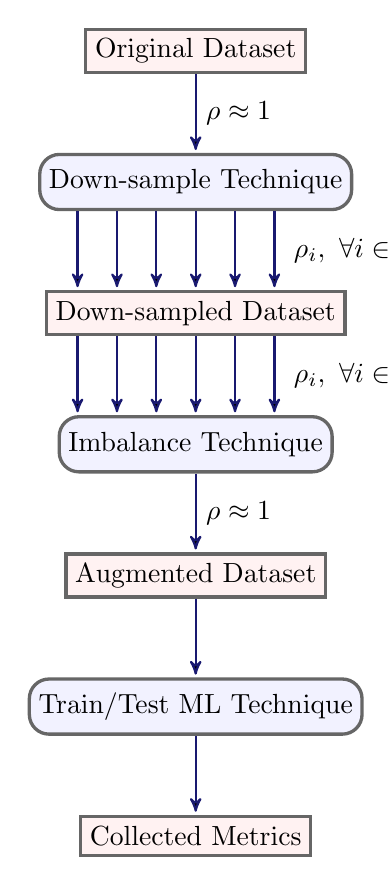
\begin{tikzpicture}[
		roundnode/.style={rectangle,rounded corners=0.25cm, draw=black!60, fill=blue!5, very thick, minimum size=7mm},
		squanode/.style={rectangle, draw=black!60, fill=red!5, very thick, minimum size=5mm},
		path/.style={draw=MidnightBlue, thick,->,>=stealth',shorten >=1pt}
		]
		
		% Nodes
		\node[squanode] (Maintable)     {Original Dataset};
		\node[roundnode] (Downsample) [below=of Maintable] {Down-sample Technique};
		\node[squanode] (Subset1) [below=of Downsample] {Down-sampled Dataset};
		\node[roundnode] (Subset2) [below=of Subset1] {Imbalance Technique};
		\node[squanode] (Subset3) [below=of Subset2] {Augmented Dataset};
		\node[roundnode] (TrainTest) [below=of Subset3] {Train/Test ML Technique};
		\node[squanode] (Subset4) [below=of TrainTest] {Collected Metrics};
		
		% Main Paths
		\path[path] (Maintable) edge []  node [right] {$\rho\approx1$} (Downsample);
		\path[path] (Subset2) edge []  node [right] {$\rho\approx1$} (Subset3);
		\path[path] (Subset3) edge []  node [below] {} (TrainTest);
		\path[path] (TrainTest) edge []  node [below] {} (Subset4);
		
		% Split
		\path[path] (Downsample) edge []  node [below] {} (Subset1);
		\path[path] (Downsample) edge [transform canvas={xshift=-5mm}]  node [right] {} (Subset1);
		\path[path] (Downsample) edge [transform canvas={xshift=-10mm}]  node [below] {} (Subset1);
		\path[path] (Downsample) edge [transform canvas={xshift=-15mm}]  node [below] {} (Subset1);
		\path[path] (Downsample) edge [transform canvas={xshift=5mm}]  node [right] {} (Subset1);
		\path[path] (Downsample) edge [transform canvas={xshift=10mm}]  node [right] {$\,\,\rho_i,\ \forall i\in I$} (Subset1);
		
		% Condense
		\path[path] (Subset1) edge []  node [below] {} (Subset2);
		\path[path] (Subset1) edge [transform canvas={xshift=-5mm}]  node [right] {} (Subset2);
		\path[path] (Subset1) edge [transform canvas={xshift=-10mm}]  node [below] {} (Subset2);
		\path[path] (Subset1) edge [transform canvas={xshift=-15mm}]  node [below] {} (Subset2);
		\path[path] (Subset1) edge [transform canvas={xshift=5mm}]  node [right] {} (Subset2);
		\path[path] (Subset1) edge [transform canvas={xshift=10mm}]  node [right] {$\,\,\rho_i,\ \forall i\in I$} (Subset2);

		%\node[red!50!black, font=\Huge\bfseries, rotate=45] at (image.center) {Draft};
	\end{tikzpicture}
	\caption{Process flow from the full dataset to subsets to the collected metrics.}
	\label{fig:trajectory}
\end{figure}

	To assess the influence of varying techniques on distinct values of $\rho$, we artificially induced imbalance by
	first isolating a test set, then randomly diminishing the count of the positive class in the dataset 
	until achieving the desired ratio, $\rho$. 
	A new subset was imbalanced subset was created for each round of experimentation.
	
	This newly imbalanced subset was then subjected to one of the several techniques under investigation
	decreasing the majority class for the undersampling techniques or increasing the minority for the oversampling techniques
	until the $\rho$ value is close to $1$.
	The efficacy of these techniques was gauged using a collection of classifiers limited to a concise set of hyperparameters.
	To minimize the potential impact of sample variance originating from the down-sampling process, we iterated this process multiple times and then averaged the results.

	\subsubsection{$k$-Nearest Neighbor}
	Following an extensive preliminary assessment of $k$ values, we discerned that a range of 1 to 20 consistently yielded moderately satisfactory results. In each iteration of experimentation involving $k$NN, a grid search methodology was executed, focusing on the odd values within the 1 to 21 range. The best-performing model emerging from this process was then selected for evaluation on the test set. The associated $k$ and F1 values for this model were collated from both the training and testing sets.

	\subsubsection{Decision Tree}
	We employed a grid search to allow for adaptability in decision tree configurations during our experiments. Initially, a full tree was fitted to the data under consideration. We then noted the maximum depth and the number of significant features. The grid hyperparameters subjected to testing spanned a range from 1 up to these recorded values. Subsequently, the top-performing model was chosen for the testing phase. The results included the maximum depth, maximum features, along with the F1 scores for both training and testing phases.

	\subsubsection{Random Forest}
	In the case of the random forest, the parameters under evaluation encompassed a range of trees, specifically 15, 20, 30, 40, 50, 100, 150, 200, 300, and 400. To expedite the generation of models during the testing of each hyperparameter, a warm start approach was employed. Upon completion of each test, we recorded the best-performing model's number of trees ($n$), along with its F1 scores.
	
	\subsubsection{Extra Trees}
	The Extra Trees test employed a parameter range identical to that utilized in the Random Forest experiments, with the addition of bootstrap sampling. Consistent with the methodology adopted for all preceding models, the corresponding parameters and F1 scores were comprehensively documented and returned for further analysis.


\subsection{Data Level Techniques}

	The methodologies adopted in this study are fundamentally data-driven, 
	divided into two primary categories: undersampling and oversampling techniques. 
	The undersampling approaches encompass Random Undersampling, Tomek Links, One-Sided Undersampling, and Near-Miss Undersampling. 
	Correspondingly, the oversampling strategies comprise Random Oversampling, SMOTE (Synthetic Minority Oversampling Technique), BorderlineSMOTE, and ADASYN (Adaptive Synthetic Sampling). 
	The intuition of these techniques can be found in Section \ref{sec:related_work} of this report, providing a foundational understanding of their theoretical underpinnings.
		

\subsection{Algorithm Level Techniques}

	The algorithmic level techniques were trained on the synthetically imbalanced instances of the datasets.
	The techniques that were tested in this experiment were the Focal Cross-entropy Loss,
	Very Deep Convolutional Neural Network, and cost-sensitive loss.
	For each technique and each round of testing the training history was collected
	and the final performance on the test data was collected to be evaluated against the
	corresponding $\rho$.

\begin{comment}
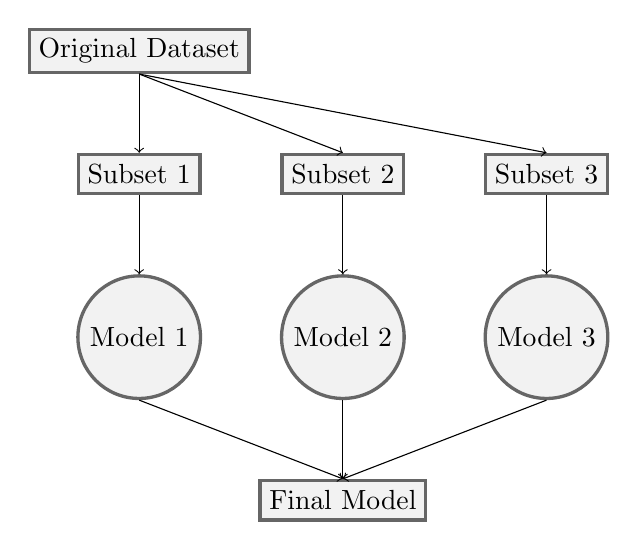
\begin{tikzpicture}[
	roundnode/.style={circle, draw=black!60, fill=black!5, very thick, minimum size=7mm},
	squanode/.style={rectangle, draw=black!60, fill=black!5, very thick, minimum size=5mm},
	]
	
	%Nodes
	\node[squanode] (Maintable)     {Original Dataset};
	\node[squanode] (Subset1) [below=of Maintable] {Subset 1};
	\node[squanode] (Subset2) [right=of Subset1] {Subset 2};
	\node[squanode] (Subset3) [right=of Subset2] {Subset 3};
	\node[roundnode] (Model1) [below=of Subset1] {Model 1};
	\node[roundnode] (Model2) [below=of Subset2] {Model 2};
	\node[roundnode] (Model3) [below=of Subset3] {Model 3};
	\node[squanode] (FinalModel) [below=of Model2] {Final Model};
	
	%Lines
	\draw[->] (Maintable.south) -- (Subset1.north);
	\draw[->] (Maintable.south) -- (Subset2.north);
	\draw[->] (Maintable.south) -- (Subset3.north);
	\draw[->] (Subset1.south) -- (Model1.north);
	\draw[->] (Subset2.south) -- (Model2.north);
	\draw[->] (Subset3.south) -- (Model3.north);
	\draw[->] (Model1.south) -- (FinalModel.north);
	\draw[->] (Model2.south) -- (FinalModel.north);
	\draw[->] (Model3.south) -- (FinalModel.north);
	
\end{tikzpicture}

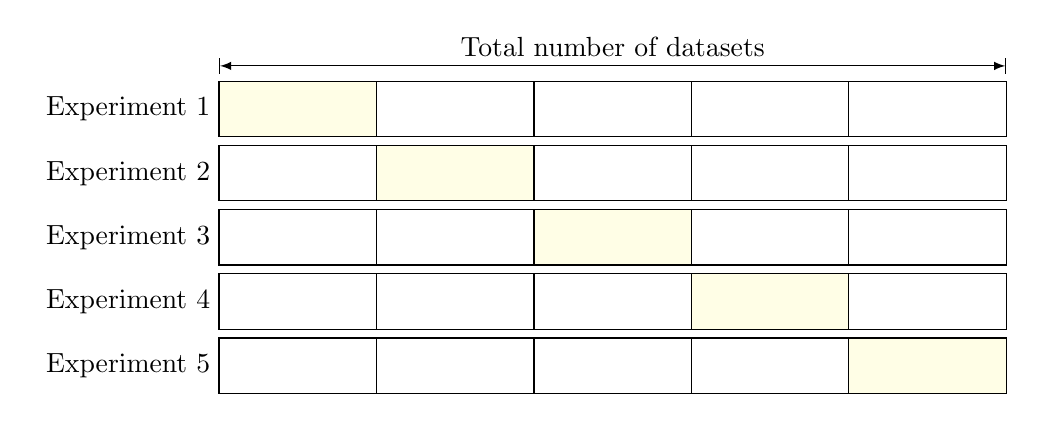
\begin{tikzpicture}
\matrix (M) [matrix of nodes,
nodes={minimum height = 7mm, minimum width = 2cm, outer sep=0, anchor=center, draw},
column 1/.style={nodes={draw=none}, minimum width = 4cm},
row sep=1mm, column sep=-\pgflinewidth, nodes in empty cells,
e/.style={fill=yellow!10}
]
{
	Experiment 1 & |[e]| & & & & \\
	Experiment 2 & & |[e]| & & & \\
	Experiment 3 & & & |[e]| & & \\
	Experiment 4 & & & & |[e]| & \\
	Experiment 5 & & & & & |[e]| \\
};
\draw (M-1-2.north west) ++(0,2mm) coordinate (LT) edge[|<->|, >= latex] node[above]{Total number of datasets} (LT-|M-1-6.north east);
\end{tikzpicture}

\end{comment}


	% Results and Discussion
	\section{Results and Discussion}
	\label{sec:results_discussion}
	
	Our exploration into different class imbalance handling techniques has led to some intriguing findings. Here, we discuss the outcomes and implications of our experiments. 6200 experiments were repeated with distinct random subsets.
	
	\subsection{Oversampling Techniques}
	
	Among the oversampling techniques evaluated, all exhibited a significant divergence between performance during the training and cross-validation stages and the results on the test sets. This disparity underscores the need for caution when relying solely on training and cross-validation metrics for model evaluation. It suggests that oversampling can potentially lead to overoptimistic estimates of model performance during training and validation phases. Consequently, it is essential to validate the model's performance using a separate test set that has not been subjected to oversampling.
	
	The evaluation of oversampling techniques can be observed through several key figures. The test F1 scores are portrayed in Figure \ref{fig:oversampling-test}, illustrating the performance of the models when presented with unseen data. Complementing this, Figure \ref{fig:oversampling-training} presents the training F1 scores, delineating the ability of the models to learn from the training dataset. The computational efficiency of the models, measured through runtime, is highlighted in Figure \ref{fig:oversampling-runtime}.
	
	Distinct banding patterns noticeable in these figures can be attributed to the varying operational times of the classifiers. An unexpected deviation in the performance of Borderline SMOTE is discernible, manifesting as an arch of unusual results. Although the precise reason behind this anomaly remains unclear, it is conjectured that it could be an artifact of shared resources within our testing environment. Further exploration will be essential to understand and address this anomalous behavior.
	
\begin{figure}
	\centering
	\includegraphics[width=0.9\linewidth]{Images/Oversampling-Test}
	\caption{Oversampling Techniques - Test F1}
	\label{fig:oversampling-test}
\end{figure}
	
\begin{figure}
	\centering
	\includegraphics[width=0.9\linewidth]{Images/Oversampling-Training}
	\caption{Oversampling Techniques - Training F1}
	\label{fig:oversampling-training}
\end{figure}

\begin{figure}
	\centering
	\includegraphics[width=0.9\linewidth]{"Images/Oversampling Runtime"}
	\caption{Oversampling Experiment Runtime}
	\label{fig:oversampling-runtime}
\end{figure}
	
	\subsection{Undersampling Techniques}
	
	For undersampling methods, Tomek Links and One-Sided Undersampling showed a much closer alignment between training and test set performance. This consistency indicates that these techniques may provide a more reliable estimate of true model performance during the training phase, reducing the risk of overfitting.
	
	Upon examining our findings, as seen in Figures \ref{fig:undersampling-test} and \ref{fig:undersampling-training}, it becomes evident that the Tomek Links and One-Sided Undersampling techniques demonstrate a distinct edge in providing a more accurate evaluation of the model's predictive performance once deployed. This advantage can primarily be attributed to their characteristic of preserving information within the data.
	
	Firstly, let's consider the impact of Tomek Links. This technique aims to identify and eliminate certain instances of the majority class that are near-neighbors to instances of the minority class. By doing so, it subtly refines the decision boundaries within the data, fostering a more distinct separation between the classes. This mechanism leads to an enhancement in the quality of the feature space representation. Hence, the model trained using Tomek Links appears to be more adept at predicting unseen data, as it has been schooled on a dataset that mirrors a more genuine depiction of the class distribution in the broader population.
	
	Similarly, One-Sided Undersampling also shows the propensity to yield a more realistic portrayal of the model's eventual predictive ability. This technique works by selectively pruning instances of the majority class that might induce overlapping and confusion between classes. By ensuring that the remaining majority instances are those that maintain a safe distance from the minority instances, One-Sided Undersampling promotes the creation of cleaner and more distinct class boundaries. Consequently, models trained using this undersampling technique are apt to make more accurate predictions on new data.
	
	The salient feature of both these techniques is their emphasis on preserving information within the dataset. Unlike some other resampling techniques that might aggressively oversample the minority class or undersample the majority class, Tomek Links and One-Sided Undersampling show a measure of restraint. They carefully curate the instances to be removed such that most of the original information is retained, particularly from the minority class. This aspect seems to be a significant contributor to their efficacy in realistically evaluating the predictive capability of the trained models.
	
	On the other hand, Random Undersampling and Near-Miss demonstrated heteroscedastic behavior, maintaining a consistent mean F1 score while exhibiting increasing variance with rising $\rho$ values. This finding suggests that while these methods may provide a stable average performance, the model's actual performance may vary significantly, particularly as class imbalance increases.

	Contrasting the aforementioned techniques, Random Undersampling and Near Miss do not seem to embody the same emphasis on information preservation. This difference could potentially provide an explanation for the observed variability in the training scores for these methods, rather than a discernable trend in any particular direction.
	
	In essence, both Random Undersampling and Near Miss appear to discard potentially crucial information during their process, unlike Tomek Links and One-Sided Undersampling. This divergence could be the root cause for the increasing variance in training scores rather than a pronounced trend in any specific direction. Therefore, our analysis further highlights the necessity of carefully considering the information preservation quality of the techniques utilized to handle class imbalance in datasets.
	
	Upon examining the runtimes for the undersampling techniques, we observe a similar banding pattern contingent on the classification method. However, a possible advantage emerges in relation to the value of $\rho$. As $\rho$ escalates, leading to a more intense undersampling procedure, there is a corresponding reduction in the overall runtime.
	
	In scenarios where pertinent information is retained effectively, this decrease in sample size may offer considerable benefits. This runtime efficiency might not only expedite the model building process, but also could potentially improve the feasibility of incorporating more complex or computationally demanding models into the classification task. Moreover, in real-world applications where time and computational resources are often limited, this efficiency gain can be of immense importance.
	
	Therefore, while the primary objective of undersampling techniques is to address class imbalance, these methods may concurrently provide the advantageous side effect of enhancing computational efficiency. This aspect underscores the multifaceted benefits of intelligently implementing undersampling techniques in machine learning tasks, reinforcing their value beyond simply addressing imbalanced datasets.	

\begin{figure}
	\centering
	\includegraphics[width=0.9\linewidth]{Images/Undersampling-Test}
	\caption{Undersampling Techniques - Test F1}
	\label{fig:undersampling-test}
\end{figure}
	
\begin{figure}
	\centering
	\includegraphics[width=0.9\linewidth]{Images/Undersampling-Training}
	\caption{Undersampling Techniques - Training F1}
	\label{fig:undersampling-training}
\end{figure}

\begin{figure}
	\centering
	\includegraphics[width=0.9\linewidth]{"Images/Undersampling Runtime"}
	\caption{Undersampling Experiment Runtime}
	\label{fig:undersampling-runtime}
\end{figure}
	
	\subsection{Algorithmic Techniques}
	
	Figures \ref{fig:cv-train-loss} and \ref{fig:cv-train-acc} show the mean and standard deviation of the loss and accuracy history when training the different models.
	
	\begin{figure}
		\centering
		\includegraphics[width=0.9\linewidth]{"Images/CV Train Loss"}
		\caption{}
		\label{fig:cv-train-loss}
	\end{figure}
	
\begin{figure}
	\centering
	\includegraphics[width=0.9\linewidth]{"Images/CV Train Acc"}
	\caption{}
	\label{fig:cv-train-acc}
\end{figure}
	
	Figures \ref{fig:cv-val-loss} and \ref{fig:cv-val-acc} show the mean and standard deviation of the loss and accuracy history relating to the validation
	set during the training of the different models.

	
\begin{figure}
	\centering
	\includegraphics[width=0.9\linewidth]{"Images/CV Val Loss"}
	\caption{}
	\label{fig:cv-val-loss}
\end{figure}
	
	
\begin{figure}
	\centering
	\includegraphics[width=0.9\linewidth]{"Images/CV Val Acc"}
	\caption{}
	\label{fig:cv-val-acc}
\end{figure}
	
	Figures \ref{fig:cv-final-loss} and \ref{fig:cv-final-accuracy} the mean and standard deviation of the model's prediction loss and accuracy
	as compared to the different values of $\rho$.
		
	
\begin{figure}
	\centering
	\includegraphics[width=0.9\linewidth]{"Images/CV FInal Loss"}
	\caption{}
	\label{fig:cv-final-loss}
\end{figure}

\begin{figure}
	\centering
	\includegraphics[width=0.9\linewidth]{"Images/CV Final Accuracy"}
	\caption{}
	\label{fig:cv-final-accuracy}
\end{figure}
	
	Overall, our findings reinforce the notion that handling class imbalance is a complex task that requires careful selection and evaluation of techniques based on the specific characteristics of the dataset and the learning algorithm. There is no one-size-fits-all solution, and the choice of technique should be guided by a thorough understanding of the underlying methods and a careful validation of the model's performance.
	
	Our study also highlights the importance of a comprehensive validation strategy that includes an assessment of the model's performance on a separate test set, particularly when oversampling techniques are used. Further research is needed to explore more sophisticated techniques, including combination methods that leverage the strengths of both oversampling and undersampling, and algorithmic level methods that modify the learning process itself to handle class imbalance.
	
	
	
	% Conclusion
	\section{Conclusion}
	\label{sec:conclusion}
	
	The investigation presented in this paper has shed light on several key aspects of handling class imbalance in machine learning datasets. As anticipated intuitively, we found that an increase in the $\rho$ value generally led to a decrease in the performance of the ensuing model. Our goal had been to discern distinctive differences in the performance degradation across various imbalance addressing techniques.
	
	While time constraints restricted the expansion of our analysis into further scenarios, our research revealed intriguing patterns, specifically regarding the training phase's behavior. This insight emphasized the necessity for nuanced caution when establishing stopping criteria, particularly in highly imbalanced datasets.
	
	In examining oversampling techniques, we observed a marked divergence between performance during the training and cross-validation steps compared to the behavior on the test sets. This result highlights the importance of careful interpretation of training and cross-validation results when oversampling techniques are used, as they may not accurately predict test set performance.
	
	Under the umbrella of undersampling, both Tomek Links and One-Sided Undersampling demonstrated a performance during training and cross-validation that was more reflective of the results achieved during testing. In contrast, Random Undersampling and Near-Miss exhibited heteroscedastic behavior. While maintaining a consistent mean F1 score, we noted an increase in variance as $\rho$ escalated.
	
	In the realm of algorithmic techniques, those that implemented cost weights seemed to yield the best final accuracy. In most cases this was contrary to the results obtained In the context of algorithmic methodologies, techniques employing cost weights consistently demonstrated superior accuracy in the final evaluations. Interestingly, these outcomes often diverged from the trends observed during the training and validation phases.
	
	We believe the findings presented here will provide valuable groundwork for further investigation into this critical area of machine learning.
	
	
	\subsection{Future Work}
	
	While our current study provides valuable insights into class imbalance handling techniques, it also paves the way for an array of future research directions.
	
	One crucial aspect of our future work involves incorporating non-random subsetting. The intent is to assess the performance of the various techniques in the context of samples that are less representative. This expansion is intended to provide a more nuanced understanding of the applicability and effectiveness of these methods across varying dataset conditions.
	
	Additionally, our plan is to incorporate additional models to perform wider evaluations. We anticipate that this extension will reinforce the robustness of our findings and allow for a more comprehensive appraisal of techniques for handling class imbalance. There remain many more techniques that can be implemented and evaluated.
	
	Through the planned future works, we aim to continue refining and extending our understanding of class imbalance solutions in machine learning, and by doing so, contribute to the field's continued advancement.
	
		
	% References
	\label{sec:references}
	\bibliographystyle{IEEEtran}
	\bibliography{Project.bib}
	
\end{document}
